% !TeX spellcheck = cs_CZ
%=========================== Kapitola: Algebra =====================================================
\setchaptertoc
\chapter{Algebra}\label{fyz:IchapXXII}
  \section{Sčítání a násobení}\label{fyz:IchapXXIIsecI}
    Při studiu kmitavých soustav budeme mít příležitost použít jednoho z nejpozoruhodnějších, přímo
    překvapujících vzorců celé matematiky. Z hlediska fyziky by nám stačilo, abychom tento vzorec
    během dvou minut uvedli a mohli bychom být spokojeni. Vědu však máme stejně tak pro
    intelektuální potěšení, jako pro praktické využití, takže místo toho, abychom tomuto vzácnému
    skvostu věnovali jen několik minut, vložíme ho přiměřeně do velkolepého rámce té části
    matematiky, jež se nazývá elementární algebrou.
    
    Možná si klademe otázku: „Co dělá matematika na přednáškách z fyziky?“ Máme k tomu několik
    možných zdůvodnění: Za prvé, je jasné, že \emph{matematika je důležitým nástrojem}, ale to by
    byl důvod jen k uvedení zmíněného vzorce ve dvou minutách. Na druhé straně, v teoretické fyzice
    objevujeme, že všechny fyzikální zákony lze napsat v matematické formě, a pociťujeme, že v tom
    je určitá jednoduchost, a proto i krása. Nakonec, abychom uměli chápat přírodu, může být
    nevyhnutelné, abychom lépe chápali matematické vztahy. Skutečný důvod je však ten, že je to
    předmět, který se nám líbí, a ačkoli si my lidé dělíme přírodu různými způsoby a na různých
    katedrách studujeme různé předměty, takovéto dělení je ve skutečnosti umělé a měli bychom se
    věnovat tomu, co nás intelektuálně těší, ať to najdeme kdekoli.
    
    Další důvod, proč se nyní chceme podrobněji věnovat algebře, ačkoli většina z nás ji studovala
    na školách nižšího stupně, je ten, že tehdy jsme ji studovali poprvé; všechny vzorce nám byly
    neznámé a byla to těžká práce. Taková, jakou máme nyní s fyzikou. Častokrát je nám potěšením
    podívat se zpět, jakou část předmětu jsme již zvládli a jak vypadá mapa nebo plán studia
    předmětu jako celku. Snad jednou někdo z katedry matematiky bude přednášet mechaniku takovým
    způsobem, aby ukázal, co jsme se snažili naučit na přednáškách z fyziky!
    
    Nebudeme se exaktně věnovat algebře z hlediska matematiky, neboť matematici se zajímají zejména
    o to, jak dokazovat různá matematická tvrzení, kolik předpokladů je absolutně nevyhnutelných a
    co není potřebné. O výsledky toho, co dokázali, se už tak nezajímají. Například Pythagorova
    věta, že součet čtverců nad odvěsnami pravoúhlého trojúhelníka je rovna čtverci nad přeponou, se
    nám může zdát docela zajímavá; je to zajímavý fakt, neobvykle jednoduchá věc, kterou můžeme
    ocenit, aniž bychom se zabývali problémem jejího důkazu nebo tím, jaké jsou k tomu třeba axiomy.
    Proto v tomto duchu, můžeme-li to tak říci, kvalitativně popíšeme systém \emph{elementární
    algebry}. Hovoříme o elementární algebře, neboť existuje takové odvětví matematiky, které se
    nazývá moderní algebra, kde neplatí některá pravidla (například \(ab = ba\)). Tou se však
    nebudeme zabývat.
    
    Diskuzi tohoto předmětu začneme od prostředka. Předpokládáme, že už víme, co jsou přirozená
    čísla, co je nula a co znamená zvětšit nějaké číslo o jednotku. Třeba si řekneme: „To není
    prostředek, to jsou začátky!“ Ale z matematického hlediska to je „prostředek“, neboť bychom se
    mohli vrátit ještě dále nazpět k teorii množin a odvodit některé z těchto vlastností přirozených
    čísel. My však nepůjdeme tímto směrem, směrem matematické filozofie a matematické logiky, ale
    vyjdeme z předpokladu, že víme, co jsou to přirozená čísla, a že s nimi umíme počítat.
    Vyjdeme-li z určitého čísla \(a\) a postupně k němu \(b\)-krát přičteme jednotku, číslo, které
    dostaneme, nazýváme \(a + b\) a tak se definuje \textbf{sčítání přirozených čísel}.
    
    Když už máme definici součtu, můžeme uvažovat takto: Začneme-li z ničeho a přičítáme k tomu
    \(b\)-krát za sebou \(a\), výsledek nazýváme \textbf{násobením přirozených čísel}; \(a\) krát
    \(b\).
    
    Dále můžeme mít i posloupnost násobení. Začneme-li s 1 a násobíme ji \(a\) \(b\)-krát za sebou,
    nazýváme to \textbf{umocňováním \(a\) na mocnitel \(b\)} tedy \(a^b\).
    
    Lze snadno dokázat, že jako výsledek těchto definic platí:
    \begin{subequations}\label{fyz:eq647}
      \begin{align}
        a+b       &=   b+a          \label{fyz:eq647a}\\
        a+(b + c) &=  (a+b)+c       \label{fyz:eq647b}\\
        ab        &=    ba          \label{fyz:eq647c}\\
        a(b + c)  &=  ab + ac       \label{fyz:eq647d}\\
        (ab)c     &=  a(bc)         \label{fyz:eq647e}\\
        (ab)^c    &= a^cb^c         \label{fyz:eq647f}\\
        a^ba^c    &= a^{(b+c)}      \label{fyz:eq647g}\\
        {(a^b)}^c &= a^{(bc)}       \label{fyz:eq647h}\\
        a + 0     &=    a           \label{fyz:eq647i}\\
        a\cdot1   &=    a           \label{fyz:eq647j}\\
        a^1       &=    a           \label{fyz:eq647k}
      \end{align}
    \end{subequations}
    Tyto vztahy jsou nám všechny dobře známé, proto je jen uvádíme. Vidíme, že \num{1} a \num{0}
    mají zvláštní vlastnosti. Například \(a + 0\) je \(a\), \(a\)-krát \num{1} = \(a\) a \(a^1\) je
    \(a\).
    
    V naší diskuzi musíme předpokládat několik dalších vlastností jako spojitost a uspořádanost, jež
    lze těžko definovat - to přenecháme rigorózní teorii. Je třeba přiznat, že jsme tu uvedli příliš
    mnoho „pravidel“. Některá z nich lze odvodit z ostatních, ale tím se nebudeme znepokojovat.
  
  \section{Inverzní operace}\label{fyz:IchapXXIIsecII}
    K těmto přímým operacím sčítání, násobení a umocňování existují i inverzní operace, jež jsou
    definovány takto: Předpokládejme, že máme dáno \(a\) a \(c\). Chceme najít hodnoty \(b\), jež
    vyhovují takovým rovnicím jako \(a + b = c\), \(ab = c\), \(b^a = c\). Je-li \(a + b = c\), pak
    \(b\) je definováno jako \(c - a\), což se nazývá \textbf{odečítání}. Operace, kterou nazýváme
    dělení, je rovněž jasná: je-li \(ab = c\), pak \(b = c/a\) definuje \textbf{dělení} - „obrácené
    “ řešení rovnice \(ab = c\). Nyní máme mocninu \(b^a = c\) a klademe si otázku: „Čemu je rovno
    \(b\)?“ Přece \(a\)-té odmocnině z \(c\), tj. \(b = \sqrt[a]{c}\). Položíme-li si například
    takovouto otázku: „Třetí mocnina kterého čísla je rovna 8?“, odpověď zní- „Třetí odmocnina z 8
    je 2.“ Protože \(b^a\) a \(a^b\) si nejsou rovny, jsou s umocňováním spojeny dva inverzní
    problémy. Druhý inverzní problém je: „Na kterou mocninu musíme umocnit 2, abychom dostali 8?
    “Tomu se říká hledání \textbf{logaritmu}. je-li \(a^b = c\), pak píšeme \(b=\log_ac\). Fakt, že
    tento zápis je komplikovanější než ostatní neznamená, že je méně elementární (alespoň v případě,
    kdy jde o celá čísla). Ačkoli se logaritmy v algebře vyučují později, ve skutečnosti jsou stejně
    jednoduché jako odmocniny; představují prostě druh řešení algebraické rovnice. Přímé a inverzní
    operace lze shrnout následujícím způsobem:

    \begin{equation}\label{fyz:eq648}
      \begin{aligned}[c]
        a + b &= c  \\[0.5em]
        ab    &= c  \\[0.5em]
        b^a   &= c  \\
        a^b   &= c  
      \end{aligned}
        \qquad\Longleftrightarrow\qquad
      \begin{aligned}[c]
            b &= c -a         \\
            b &= \frac{c}{a}  \\
            b &= \sqrt[a]{c}  \\
            b &= \log_ac.  
      \end{aligned}
    \end{equation}
   
    Zde jsme u jádra věci. Tyto vztahy nebo pravidla platí pro přirozená čísla, neboť vyplývají z
    definic sčítání, násobení a umocňování. Chceme zjistit, zda \emph{můžeme nebo nemůžeme rozšířit
    třídu objektů, jež představují \(a\), \(b\), a \(c\), aby pro neplatila stejná pravidla}, ačkoli
    procesy sčítání \(a + b\) atd. už nebude možno definovat například ve smyslu přímého přičítání 1
    nebo postupného násobení přirozenými čísly.
  
  \section{Abstrakce a zobecnění}\label{fyz:IchapXXIIsecIII}
    Při řešení algebraických rovnic použitím všech těchto definic brzy objevíme neřešitelné problémy,
    takové, jako je tento: Předpokládejme, že chceme vyřešit rovnici \(b= 3-5\). Znamená to, že
    podle naší definice odčítání musíme najít číslo, které, když ho přičteme k \num{5}, dává \num{3}.
    Přirozeně, takové číslo neexistuje, neboť v úvahu bereme jen přirozená čísla - je to neřešitelný
    problém. Východiskem je však zajímavý plán, velkolepá myšlenka: abstrakce a zobecnění. Z celé
    struktury algebry (pravidla plus přirozená čísla) abstrahujeme původní definice sčítání a
    násobení, ale ponecháváme si pravidla (\ref{fyz:eq647}) a (\ref{fyz:eq648}), o nichž budeme
    předpokládat, že platí pro širší třídu čísel, i když byly původně odvozeny pro užší třídu čísel.
    Tedy místo toho, abychom použili přirozená čísla k definování pravidel, použijeme tato pravidla k
    definici symbolů, jež představují nějaký obecnější druh čísel. Například použitím jen samotných
    pravidel můžeme dokázat, že \(3-5=0-2\). Skutečně můžeme dokázat, že všechna odčítání lze
    provést, definujeme-li celou množinu nových čísel: \(0-1\), \(0-2\), \(0-3\), \(0-4\) atd., tzv.
    \textbf{záporná celá čísla} (\emph{negative integers}). Pak můžeme uvažovat o všech dalších
    pravidlech jako \(a(b+a)=ab+ac\) a podobně a zjišťovat, jak tato pravidla vypadají pro záporná
    čísla. Zjistíme, že všechna pravidla jsou platná pro záporná i pro kladná celá čísla.
    
    Takže rozsah objektů, pro něž platí pravidla, jsme zvětšili, ale změnil se význam symbolů.

    Nelze například říci, že \num{-2} krát \num{5} znamená \num{-2} krát přičíst \num{5}. To nemá
    smysl, ale přesto bude všechno vycházet podle pravidel.

    Zajímavý problém vzniká při umocňování. Předpokládejme, že chceme zjistit, co znamená
    \(a^{(3-5)}\). Víme jen, že \(3-5\) je řešením úlohy \((3-5)+5=3\). Odtud víme, že
    \(a^{(3-5)}a^5 = a^3\). Proto podle definice dělení \(a^{(3-5)} = \frac{a^3}{a^5}\). Dáme-li si
    trochu práce, dostaneme výsledek ve tvaru \(\frac{1}{a^2}\), takže vidíme, že záporné mocniny
    jsou reciproké ke kladným mocninám, ale symbol \(\frac{1}{a^2}\) zatím nemá smysl, neboť, ať už
    je a kladné nebo záporné, jeho druhá mocnina je číslo větší než \num{1} a ještě nevíme, co se
    myslí tím, když 1 dělíme číslem větším než \num{1}!

    Pojďme dále. Naším plánem je pokračovat v procesu zobecňování. Vždy, když najdeme další problém,
    který nemůžeme vyřešit, rozšíříme náš \textbf{číselný obor}. Vezměme si dělení: Nemůžeme najít
    takové celé číslo, dokonce ani záporné celé číslo, jež by bylo výsledkem dělení \(3:5\).
    Předpokládáme-li však, že i všechny \textbf{zlomky} splňují daná pravidla, můžeme hovořit o
    násobení a sčítání zlomků a vše vychází stejně dobře jako předtím.

    Vezměme si další příklad s mocninami: Co je \(a^\frac{3}{5}\)? Víme jen, že \(\frac{3}{5}5=3\),
    neboť to byla definice \(\frac{3}{5}\). Takže také víme, že \(a^{\frac{3}{5}5}=a^3\), neboť to je
    jedno z pravidel. Z toho pomocí definice odmocniny zjistíme, že \(a^\frac{3}{5}=\sqrt[5]{a^3}\).
    
    Tak můžeme definovat, co znamenají zlomky v různých výrazech - samotná pravidla nám pomáhají
    určit definice, není v tom libovůle. Je to pozoruhodný fakt, že všechna pravidla stále platí jak
    pro kladná a záporná celá čísla, tak i pro zlomky!

    Pokračujme v procesu zobecňování. Existují nějaké další rovnice, které neumíme vyřešit? Ano,
    existují. Například nelze vyřešit rovnici \(b=2^\frac{1}{2} =\sqrt{2}\). Není možné najít takové
    racionální číslo (zlomek), jehož druhá mocnina je rovna 2. V moderní době je na tuto otázku
    velmi snadná odpověď'. Známe desetinný systém, takže nám nedělají problémy nekonečná desetinná
    čísla jako způsob aproximace druhé odmocniny ze 2. Historicky to však byl velký problém pro
    staré Řeky. Skutečně přesná definice toho, o co tu jde, vyžaduje znát něco z podstaty spojitosti
    a uspořádanosti, a to je na tomto místě právě nejtěžší krok v procesu zobecňování. Formálně a
    velmi přesně to provedl \RichardDedekind. Avšak, bez obav o matematickou přesnost, můžeme snadno
    pochopit, co zamýšlíme provést, tj. aproximovat takové číslo celou posloupností desetinných
    zlomků (neboť každé konečné desetinné číslo je racionální číslo), která se stále více a více
    přibližuje k hledanému výsledku. To nám pro naše účely postačí, umožní nám to manipulovat s
    iracionálními čísly i jejich výpočet (jako například čísla \(\sqrt{2}\)) s libovolnou přesností.

  \section{Aproximace iracionálních čísel}\label{fyz:IchapXXIIsecIV}
    Další problém se objeví u iracionálních mocnitelů. Chceme například vědět, čemu je rovno
    \(10^{\sqrt{2}}\). Odpověď je v podstatě jednoduchá. Aproximujeme-li \(\sqrt{2}\) desetinným
    číslem s určitým počtem desetinných míst, pak mocnitel je racionální číslo a předcházející
    metodou můžeme vypočítat aproximaci čísla \(10^{\sqrt{2}}\). Dále můžeme desetinné číslo
    prodloužit o několik desetinných míst (znovu to bude racionální číslo), vypočítat příslušnou
    odmocninu (tentokrát mnohem vyšší, neboť jmenovatel zlomku je nyní mnohem větší) a dostaneme
    lepší přiblížení. Samozřejmě odmocniny, které se tu vyskytnou, budou mít vysoké odmocnitele a
    výpočet bude dost obtížný. Jak se můžeme vypořádat s tímto problémem?
  
    K výpočtu druhé odmocniny, třetí odmocniny a jiných odmocnin nižšího řádu existuje aritmetický
    postup, pomocí něhož můžeme vypočítat jedno desetinné místo za druhým. Ale námaha, již je třeba
    vynaložit při počítání iracionálních mocnin a s nimi spojených logaritmů (inverzní problém), je
    příliš velká, neboť neexistuje jednoduchý aritmetický předpis, který bychom mohli použít. Proto
    byly sestaveny tabulky, jež nám umožňují počítat takovéto mocniny. Nazývají se \textbf{tabulky
    logaritmů} nebo \textbf{tabulky mocnin} podle toho, jak jsou sestaveny. Je to jen otázka úspory
    času. Když máme umocnit nějaké číslo na iracionální mocninu, můžeme si výsledek místo počítání
    vyhledat. Příslušný výpočet je, samozřejmě, jen technickým problémem, ale je to zajímavý problém
    s dlouhou historií. V první řadě, nejen že máme problém jak vyřešit \(x=10^{\sqrt{2}}\), ale i
    to, jak vyřešit \(10^x=2\) neboli \(x= \log_{10}2\). Není to problém toho typu, kdy jsme museli
    zavádět nějaký nový druh čísel; je to čistě počtářský problém. Výsledkem je iracionální číslo s
    nekonečným počtem desetinných míst a ne nějaký nový druh čísla.

    Nyní se zabývejme otázkou řešení takových rovnic. Základní myšlenka je skutečně velmi
    jednoduchá. Vypočítáme-li \(10^1\), \(10^{4/10}\), \(10^{1/100}\), \(10^{4/1000}\) atd. a
    vynásobíme-li je navzájem, dostaneme \(10^{1.414\ldots}\), tj. \(10^{\sqrt{2}}\). To je
    základní myšlenka výpočtu. Místo počítání \(10^{1/10}\), atd. však budeme počítat \(10^{1/2}\),
    \(10^{1/2}\) atd. Předtím si však vysvětlíme, proč používáme číslo \num{10} a ne nějaké jiné
    číslo. Víme, že logaritmické tabulky jsou velmi užitečné pro praxi, neboť, odhlédneme-li od
    matematického problému výpočtu odmocnin, platí pro každý základ
    \begin{equation}\label{fyz:eq693}
      \log_b(ac)=\log_ba+log_bc.
    \end{equation}
  
    \begin{table}[ht!]
      \centering
      \resizebox{1\linewidth}{!}{
      \renewcommand{\arraystretch}{1.2}
      \begin{tabular}{@{}llll@{}}
        \toprule
        Mocnitel s  & \(1024s\) & \multicolumn{1}{c}{\(10^s\)}   & \((10^s−1)/s\)  \\\midrule
        1           & 1024      & \num{10.00000 }   & \(\num{9.00  }    \)         \\
        1/2         & 512       & \num{3.16228  }   & \(\num{4.32  }    \)         \\
        1/4         & 256       & \num{1.77828  }   & \(\num{3.113 }    \)         \\
        1/8         & 128       & \num{1.33352  }   & \(\num{2.668 }    \)         \\
        1/16        & 64        & \num{1.15478  }   & \(\num{2.476 }    \)         \\
        1/32        & 32        & \num{1.074607 }   & \(\num{2.3874}    \)         \\
        1/64        & 16        & \num{1.036633 }   & \(\num{2.3445}    \)         \\
        1/128       & 8         & \num{1.018152 }   & \(\num{2.3234}^{211}\)       \\
        1/256       & 4         & \num{1.0090350}   & \(\num{2.3130}^{104}\)       \\
        1/512       & 2         & \num{1.0045073}   & \(\num{2.3077}^{53} \)       \\
        1/1024      & 1         & \num{1.0022511}   & \(\num{2.3051}^{26} \)       \\
                    &           &                   & \multicolumn{1}{c}{\(\downarrow^{26}\)}    \\
        \(Δ\)/1024  & \(Δ\)     & 1+0.0022486 \(Δ\) & \(\num{2.3025}\)            \\
        (\(Δ\rightarrow0\)) &   &                   &                             \\\bottomrule   
      \end{tabular}
      }
      \caption{Postupně druhé odmocniny čísla \num{10}}
      \label{fyz:tab011}
    \end{table}

    Všichni víme, že tento vztah lze výhodně použít při výpočtu součinů použitím logaritmických
    tabulek. Jedinou otázkou je, s jakým základem \(b\) máme počítat? Na tom nezáleží, vždyť tento
    vztah stále platí a použijeme-li logaritmy s nějakým základem, můžeme logaritmy pro jakýkoli
    jiný základ najít jednoduše změnou škály - vynásobením nějakým faktorem. Vynásobíme-li rovnici
    (\ref{fyz:eq693}) číslem \num{61}, pak bude platit stejně; proto výsledek bude stejný, ať
    použijeme tabulky logaritmů pro základ \(b\) nebo tabulky, kdy všechny logaritmy byly vynásobeny
    číslem \num{61}. Předpokládejme, že známe logaritmy se základem \(b\) pro všechna čísla, tj. že
    známe řešení rovnice \(b^a = c\) pro jakékoli \(c\). Čemu je roven logaritmus stejného čísla při
    jiném základu, řekněme při základu \(x\)? Odpověď najdeme řešením rovnice \(x^{a'} = c\), což
    provedeme snadno, neboť vždy můžeme psát \(x = b^t\). Tento vztah nám definuje \(t\) při známém
    \(x\) a \(b\) takto: \(t= \log_bx\). Dosadíme-li \(b^t\) za \(x\), máme \((b^t)^{a'}=b^{ta'} =
    c\), jinými slovy, \(ta'\) je logaritmus \(c\) s bází \(b\), a proto \(a' =a/t\). Takže
    logaritmy se základem \(x\) jsou rovny logaritmům se základem b, jež vynásobíme konstantou
    \(1/t\). Libovolné dvě tabulky logaritmů jsou ekvivalentní, vynásobíme-li jednu z nich
    konstantou \(1/\log_bx\). To nám umožňuje zvolit si libovolný základ. Z praktických důvodů
    bereme za základ číslo 10. (Může vzniknout otázka, zda neexistuje nějaký přirozený základ, pro
    který se věci zjednoduší. Odpověď na tuto otázku se pokusíme najít později. Prozatím budeme
    používat jako základ číslo 10.)

    Podívejme se, jak se počítají logaritmy. Začneme výpočtem postupných odmocnin čísla \num{10}.
    Výsledky jsou v tab. \ref{fyz:tab011}. Mocnitele čísla \num{10} jsou v prvním sloupci a mocniny
    \(10^s\) jsou ve třetím sloupci. Máme \(10^1 = 10\). Deset na jednu polovinu můžeme snadno
    vypočítat, neboť to je druhá odmocnina z \num{10} a druhou odmocninu jakéhokoli čísla lze snadno
    vypočítat\footnote{ Existuje k tomu určitý aritmetický algoritmus, ale nejjednodušší způsob, jak
    najit druhou odmocninu jakéhokoli čísla \(N\), je vzít si její přibližnou hodnotu \(a\), najít
    \(N/a\), udělat průměr \(a' =\frac{(a + N/a)}{2}\) a toto \(a'\) si vzít jako novou hodnotu pro
    \(a\). Konvergence je velmi rychlá - počet platných desetinných míst se vždy zdvojnásobí.}

    Hledaná odmocninaje \num{3.16228}. K čemu je to dobré? Již tento výsledek nám něco říká; známe
    už alespoň jeden logaritmus; kdybychom potřebovali logaritmus \num{3.162278}, pak víme, že
    výsledek je velmi blízko k \num{0.500 00}. Potřebujeme se však dostat dále; potřebujeme více
    informací. Proto najdeme znovu druhou odmocninu, čímž dostaneme \(10^{1/4}\), což je
    \num{1.77828}. Nyní známe logaritmus více čísel: \num{1.250} je logaritmus \num{17.78} a shodou
    okolností, chce-li někdo vědět čemu je rovno \num{10e0.75}, můžeme to vypočítat, neboť to je
    \(10^{(0.5+0.25)}\) , a tedy je to součin druhého a třetího čísla v tabulce \ref{fyz:tab011}.
    Budeme-li mít ve sloupci mocnitelů dostatečně mnoho čísel, abychom z nich mohli zkombinovat
    téměř každé číslo, můžeme vynásobením příslušných čísel ve třetím sloupci najít libovolnou
    mocninu 10, a o to nám jde. Najdeme tedy deset opakovaných druhých odmocnin 10 a to je hlavní
    část našeho výpočtu.

    Proč nepokračujeme dále ve zvyšování přesnosti tabulky? Protože jsme si něčeho všimli.
    Umocníme-li \num{10} na velmi malou mocninu, dostaneme 1 plus malé číslo. Proč je to tak, je
    jasné, neboť chceme-li z \(10^{1/1000}\) dostat znovu \num{10}, musíme najít tisící mocninu,
    takže je lépe nezačínat s příliš velkými čísly. Odmocniny s příliš velkými odmocniteli budou
    blízké jedné. Vidíme, že malá čísla, která jsou přičtena k 1, se začínají zmenšovat, jako
    kdybychom je vždy vydělili 2. Vidíme, že \num{1815} přejde na \num{903}, potom na \num{450},
    \num{225} atd. Vypočteme-li tedy další odmocninu, dostaneme \num{1.00112} ve výborném přiblížení
    a místo výpočtu všech dalších odmocnin odhadneme konečnou limitu. Čemu bude rovno 10 umocněno na
    malou část \(\Delta\) z \num{1024}, když se \(\Delta\) blíží k nule? Bude to nějaké malé číslo,
    blízké \num{0.0022511} \(\Delta\). Nebude to přesně tato hodnota, ale přesnější hodnotu můžeme
    určit takovýmto trikem: Od \(10^s\) odečteme 1 a vydělíme mocnitelem \(s\). Tím se všechny malé
    odchylky od 1 budou blížit ke stejnému číslu. Vidíme, že jsou si velmi blízké. Na začátku
    čtvrtého sloupce tabulky si sice nejsou rovny, ale jak postupujeme dolů, rozdíly se zmenšují,
    vždy přibližně na polovinu předcházejícího rozdílu: \num{211}, \num{104}, \num{53}, \num{26}.
    Kdybychom pokračovali, byly by \num{13}, \num{7}, \num{3}, \num{2} a \num{1} nebo dohromady
    \num{26}. Takže do konečné správné hodnoty nám chybí \num{26} a ta je proto \num{2.3025}.
    (Později se přesvědčíme, že přesná hodnota má být \num{2.3026}, ale protože jsme realisté,
    nebudeme na našem výpočtu nic měnit.) Pomocí této tabulky nyní můžeme určit jakoukoli mocninu
    čísla 10, jestliže exponent vyjádříme jako násobky \(1/1024\).

    \begin{strip}
      \begin{align}\label{fyz:eq694}
                     2&÷\num{1.77828} =\num{1.124682}                                    \nonumber\\
        \num{1.124682}&÷\num{1.074607}=\num{1.046598}                 \qquad\text{atd.}  \nonumber\\
                  ∴  2&=(\num{1.77828})\cdot(\num{1.074607})\cdot
                       (\num{1.036633})\cdot(\num{1.0090350})\cdot(\num{1.000573})       \nonumber\\
                      &=10^{\left[\dfrac{1}{1024}(256+32+16+4+\num{0.254})\right]}
                       =10^{\left[\dfrac{308.254}{1024}\right]}                          \nonumber\\
                      &=10^{\num{0.30103}}\qquad\left(\frac{573}{2249}=\num{0.254}\right)\nonumber\\
          ∴ \log_{10}2&=\num{0.30103}    \qquad\rightarrow\text{výpočet logaritmu}                                       
      \end{align}
    \end{strip}

    Proveďme nyní výpočet logaritmu. Použijme postup, pomocí něhož se skutečně sestavovaly
    logaritmické tabulky. Tento postup je znázorněn v algoritmu \ref{fyz:eq694} a číselné hodnoty
    jsou vzaty z druhého a třetího sloupce tab. \ref{fyz:tab011}.

    Předpokládejme, že chceme vypočítat logaritmus čísla \num{2}, tj. chceme vědět, na jaký mocnitel
    musíme umocnit \num{10}, abychom dostali \num{2}. Můžeme umocnit \num{10} na \(1/2\)? Ne, to je
    číslo mnohem větší, než \num{2}. Vidíme tedy, že hledaný mocnitel bude větší než \(1/4\) a menší
    než \(1/2\). Vydělíme \num{2} číslem \(10^{1/4} = \num{1.778}\ldots\) a dostaneme
    \(\num{1.124}\ldots\). Tím jsme z logaritmu oddělili část rovnou \num{0.250000}. Nyní hledáme
    logaritmus čísla \(\num{1.124}\ldots\) a když ho budeme mít, přičteme k němu \(1/4\) neboli
    \(256/1024\). Dále najdeme v tabulce nejbližší číslo \(\num{1.124}\ldots\), což je číslo
    \num{1.074607}. Jím budeme dělit a dostaneme \num{1.046598}. Tak zjistíme, že \num{2} lze napsat
    jako součin těchto čísel z tab. \ref{fyz:tab011}:
    \begin{align*}
      \num{1.77828}\cdot\num{1.074607} &= \num{1.91095}                                        \\
      \num{1.91095}\cdot\num{1.036633} &= \num{1.98095}                                        \\
      \num{1.98095}\cdot\num{1.009035} &= \num{1.99885}                                        \\
      \num{1.99885}\cdot\num{1.000578} &= \num{2}.
    \end{align*}

    Poslední číslo \num{1.000573} je již mimo rozsah naší tabulky. K určení logaritmu tohoto čísla
    použijeme výsledek, že \(10^{\Delta/1024} = 1 +\num{2.3025} \Delta/1024\). Odtud máme
    \(\Delta=\num{0.254}\). Proto je třeba 10 umocnit na tuto mocninu: \((\num{256} + \num{32} +
    \num{16} + \num{4} + \num{0.254})/1024\). Sečtením dostáváme \(\num{308.254}/1024\) a po dělení
    máme \num{0.30103}, takže \(\log_{10}2 = \num{0.30103}\), což je výsledek přesný na \num{5}
    desetinných míst!

    Tímto způsobem poprvé počítal logaritmy pan Briggs z Halifaxu v r. 1620, který řekl: „Postupně
    jsem vypočítal \num{54} druhých odmocnin z čísla \num{10}“. Víme, že ve skutečností počítal jen
    prvních \num{27} odmocnin, neboť ostatní lze vypočítat pomocí našeho triku s \(\Delta\). Druhou
    odmocninu z \num{10} počítal postupně \num{27}-krát, což je o sedmnáct odmocnin víc, než jsme
    počítali my, ale dalo mu to mnohem více práce, neboť počítal až na \num{16} desetinných míst, a
    když tabulky uveřejnil, zaokrouhlil výsledky na 14 desetinných míst, proto byly bez
    zaokrouhlovacích chyb. Touto metodou vypočítal logaritmy na \num{14} desetinných míst, což bylo
    dost namáhavé, ale všechny logaritmické tabulky, jež byly vydány v průběhu dalších třista let,
    byly vypůjčeny z Briggsových tabulek, přičemž byl zredukován počet desetinných míst. Jen nedávno
    byly počítači vypočteny nové tabulky. Dnes existují mnohem efektivnější metody výpočtu logaritmů
    pomocí rozvojů do nekonečných řad.

    V předcházejících výpočtech jsme objevili velmi zajímavou věc, a to, že pro velmi malé mocniny
    \(\varepsilon\) můžeme \(10^\varepsilon\) vypočítat velmi snadno. Čistě numerickou analýzou jsme
    zjistili, že \(10^\varepsilon=1 + \num{2.3025}\varepsilon\). Samozřejmě, z toho vyplývá, že pro
    velmi malé \(n\) je \(10^{n/\num{2.3025}} =1 + n\). Také víme, že logaritmy vzhledem k
    jakémukoli jinému základu jsou násobky logaritmů se základem \num{10}. Číslo \num{10} jsme
    zvolili jako základ jen proto, že máme \num{10} prstů a snadněji se nám počítá v desítkové
    soustavě. Chceme-li však najít matematicky přirozený základ, jenž nemá nic společného s počtem
    prstů lidských bytostí, můžeme se pokusit vhodně změnit naši škálu logaritmů. Lze to provést
    tak, že logaritmy se základem \num{10} se vynásobí \(\num{2.3025}\ldots\). To odpovídá novému
    základu logaritmů, jenž se nazývá přirozeným základem a označuje se \(e\). Všimněme si, že
    \(\log_e(1 + n) = n\) neboli \(e^n \approx 1+n\) pro \(n\rightarrow0\).

    Snadno se zjistí, čemu je \(e\) rovno: \(e=10^{1/\num{2.3025}}\) neboli
    \(10^{\num{0.434294}\ldots}\), je to tedy iracionální mocnina. Naši tabulku postupných druhých
    odmocnin z \num{10} můžeme použít nejen k výpočtu logaritmů, ale i libovolných mocnin čísla
    \num{10}. Vypočtěme tedy, čemu je roven tento přirozený základ \(e\). Nejdříve přepíšeme číslo
    \(\num{0.434294}\ldots\) jako \num{444.73}/\num{1024}. Vidíme, že \(\num{444.73} =\num{256} +
    \num{128} + \num{32} + \num{16} + \num{2} + \num{0.73}\). Protože máme sumu v exponentu, bude
    \(e\) součinem čísel
    \begin{align*}
      \num{1.77828}\cdot\num{1.333520} &=\num{2.37137}        \\
      \num{2.37137}\cdot\num{1.074607} &=\num{2.54829}        \\
      \num{2.54829}\cdot\num{1.036633} &=\num{2.64164}        \\
      \num{2.64164}\cdot\num{1.018152} &=\num{2.68959}        \\
      \num{2.68959}\cdot\num{1.009035} &=\num{2.71389}        \\
      \num{2.71389}\cdot\num{1.001643} &=\num{2.71834}.
    \end{align*}
      (Jediné číslo, které není v tabulce, je \num{0.73}, ale víme, že je-li \(\Delta\) dostatečně
      malé je výsledek roven \(1+\num{2.3025}\Delta\)). Po vynásobení všech čísel máme
      \num{2.71834}. (Mělo by to být \num{2.71828}, ale i tento výsledek je dost přesný.)
      Iracionální mocniny a logaritmy se tedy počítají z takovýchto tabulek.  Tak jsme vyřídili
      iracionální čísla.\footnote{V dnešní době počítačů a kalkulaček ztratily Logaritmické tabulky
      jako nástroj] numerických výpočtů svůj význam. Feynmanovo líčení nám však dává krásnou
      představu o historické úloze logaritmů a obrovském úsilí, jež museli vynaložit vědci v
      minulých stoletích při numerických výpočtech. Feynman sám však dokázal právě popsanými
      metodami a „triky“ nacházet a odhadovat numerické výsledky zpaměti tak, že mohl dokonce
      soutěžit s tzv. \uv{zázračnými počtáři}.}

  \section{Komplexní čísla}\label{fyz:IchapXXIIsecV}     
    Navzdory dosavadní námaze stále neumíme vyřešit všechny rovnice. Například čemu je rovna druhá
    odmocnina \(z-1\)? Předpokládejme, že máme řešit rovnici \(x^2 =-1\) . Druhá mocnina žádného
    racionálního, ani iracionálního čísla, ba ani ničeho, co zatím známe, není rovna \num{-1}. Naše
    čísla musíme znovu zobecnit a jejich třídu dále rozšířit. Předpokládejme, že řešením rovnice
    \(x^2 = -1\) je něco, co nazveme \(\imath\). Toto „\(\imath\)“ má definitoricky tu vlastnost, že
    jeho druhá mocnina je rovna \num{-1}. Je to tak všechno, co o něm můžeme říci. Rovnice \(x^2 =
    -1\) má však více než jeden kořen. Někdo může řešení napsat jako \(\imath\), ale někdo jiný může
    říci: \uv{Já s tím nesouhlasím, dávám přednost \(-\imath\). Moje \(\imath\) je minus vaše
    \(\imath\)}. Také \(-\imath\) je právě tak dobré řešení; neboť jediná definice \(\imath\) je, že
    \(\imath^2 = -1\), pak musí platit, že každá rovnice, kterou napíšeme, je stejně správná,
    jestliže se v ní všude změní znaménko u \(\imath\). Tomu se říká komplexní sdružení. Pomocí
    sčítání čísel \(\imath\), jejich násobením čísly, přičítáním dalších čísel apod. podle našich
    pravidel můžeme vytvořit nová čísla. Tak zjistíme, že čísla lze zapsat ve tvaru \(p + \imath
    q\), kde \(p\) a \(q\) nazýváme reálná čísla, tj. čísla, která jsme si definovali dříve. Číslo
    \(\imath\) se nazývá imaginární jednotkou. Každý reálný násobek čísla i se nazývá \textbf{ryze
    imaginární číslo}. Nejobecnější číslo a má tvar \(p + \imath q\) a nazývá se komplexní číslo.
    Vynásobíme-li například dvě taková čísla, řekněme \((r + \imath s)(p + \imath q)\), pak se nic
    hrozného nestane. Podle našich pravidel dostaneme
    \begin{align}\label{fyz:eq697}
      (r+\imath s)(p+\imath q)&=rp+r(\imath q)+(\imath s)p+(\imath s)(\imath q)   \nonumber \\
                              &=rp+\imath(rq)+\imath(sp)+(\imath\imath)(sq)       \nonumber \\
                              &=(rp−sq)+\imath(rq+sp),
    \end{align}
    protože \(\imath\imath = \imath^2 = -1\). Proto všechna čísla, která vyhovují pravidlům
    (\ref{fyz:eq647}), mají takovýto matematický tvar.

    Třeba řeknete: „Tak bychom mohli pokračovat do nekonečna! Definovali jsme mocniny imaginárních
    čísel a to, co s tím souvisí, a když už jsme hotovi, někdo přijde s další rovnicí, kterou nelze
    řešit, jako například \(x^6 + 3x^2 = -2\), a musíme dělat další zobecnění!“ Ukazuje se však, že
    s tímto jediným dalším zobecněním (\(\imath^2 = -1)\) lze vyřešit všechny algebraické rovnice!
    Je to fantastický fakt, jehož důkaz přenecháme matematikům. Důkazy jsou velmi pěkné a zajímavé,
    ale určitě ne samozřejmě. Opravdu nejsamozřejmější by bylo předpokládat, že budeme muset
    vymýšlet stále nová čísla, ale největším překvapením je, že to není třeba. To je poslední objev
    a po zavedení komplexních čísel se můžeme přesvědčit, že původní pravidla stále platí i pro
    komplexní čísla a již nepotřebujeme vymýšlet nová čísla. Umíme vypočítat komplexní mocninu
    jakéhokoli komplexního čísla; umíme vyřešit jakoukoli algebraickou rovnici a to všechno pomocí
    konečného počtu takovýchto symbolů. Nenacházíme žádná nová čísla. Například druhá odmocnina z
    \(\imath\) má přesný význam, není to něco nového. I mocnina \(\imath^\imath\) je definována. Nyní
    se na to podíváme.

    Již jsme ukázali, jak se násobí. Sčítání je též snadné. Sčítáme-li dvě komplexní čísla \((p +
    \imath q)(r + \imath s)\), výsledek je \((p + r) + \imath(q + s)\). Již víme, jak se čísla
    sčítají a násobí, ale problémem zůstává, jak vypočítat komplexní mocniny komplexních čísel.
    Ukazuje se, že to není o nic složitější než počítání komplexních mocnin reálných čísel.
    Podívejme se proto, jak lze vypočítat komplexní mocninu čísla \num{10} (nejen iracionální
    mocninu, ale \(10^{r+\imath s}\)). Samozřejmě, stále se musíme přidržovat našich pravidel
    (\ref{fyz:eq647}) a (\ref{fyz:eq648}). Máme
    \begin{equation}\label{fyz:eq698}
      10^{(r+\imath s)}=10^r10^{\imath s}.
    \end{equation}
    Již víme, jak vypočítat \(10^r\), násobit něco něčím rovněž dokážeme, proto jediný problém je,
    jak vypočítat \(10^{\imath s}\). Nechť je \(10^{\imath s}\) rovno komplexnímu číslu \(x + \imath
    y\). Problém vypadá takto: je třeba najít \(x\) a \(y\) při daném \(s\). Jestliže
    \begin{equation*}
      10^{\imath s} = x + \imath y,
    \end{equation*}
    pak musí platit \(\imath\) komplexně sdružená rovnice
    \begin{equation*}
      10^{-\imath s} = x - \imath y,
    \end{equation*}
    (Vidíme, že použitím našich pravidel můžeme odvodit množství výsledků, aniž bychom něco
    počítali.) Vynásobením odvodíme další zajímavý výsledek
    \begin{align}
      10^{\imath s}10^{−\imath s} &=10^0=1                                     \nonumber\\
                                  &=(x+\imath y)(x−\imath y)=x^2+y^2.          \label{fyz:eq699}
    \end{align}
    Najdeme-li tedy \(x\), budeme znát i \(y\).

    Problémem zůstává, jak vypočítat imaginární mocninu čísla \num{10}. Existuje k tomu nějaký klíč?
    Můžeme si pomoci našimi pravidly a dále se nedostaneme; ale existuje tu jeden rozumný nápad.
    Budeme-li to umět pro nějaké \(s\), pak to snadno určíme pro všechna ostatní \(s\). (Známe-li
    například \(10^{\imath s}\) pro nějaké \(s\) a pak chceme znát takovouto mocninu pro dvojnásobné
    \(s\), uděláme z toho druhou mocninu a podobně.) Ale jak najít \(10^{\imath s}\), i když jen pro
    jedinou hodnotu \(s\)? Uděláme proto dodatečný předpoklad, jenž nepatří zcela do kategorie
    našich ostatních pravidel, ale jenž vede k rozumným výsledkům a umožní nám postup: je-li
    mocnitel \(\imath s\) malý, budeme předpokládat, že platí \(10^\varepsilon = 1 +
    \num{2.3025}\varepsilon\) nejen pro malá reálná \(\varepsilon\), ale i pro komplexní
    \(\varepsilon\). Vyjdeme proto z předpokladu, že obecně platí \(10^\varepsilon = 1 +
    \num{2.3025}\cdot\imath s\) pro \(s\rightarrow0\). Pak, je-li s velmi malé (řekněme \(1/1024\)),
    máme docela dobrou aproximaci čísla \(10^{\imath s}\).

    Nyní sestavíme tabulku, podle níž můžeme vypočítat všechny imaginární mocniny čísla \num{10},
    tj. příslušné \(x\) a \(y\). Začneme tím, že jako první mocnitel vezmeme \(1/1024\), o němž
    předpokládáme, že je velmi přesně roven \(1 + \num{2.3025i}/1024\), tedy 
    \begin{equation}\label{fyz:eq700}
      10^{i/1024}=\num{1.00000+0.0022486i},
    \end{equation}
  
    \begin{table}[ht!]
      \centering
      \renewcommand{\arraystretch}{1.2}
      \begin{tabular}{@{}l|lr@{}}
        \toprule
        mocnitel \(s\)   & \(\num{1024} s\)  & \multicolumn{1}{c}{\(10^{\imath s}\)}  \\ \hline
        \(\imath/1024\) & \num{1   }        &  *\(\num{+1.00000+0.00225i}\)               \\
        \(\imath/512 \) & \num{2   }        &   \(\num{+1.00000+0.00450i}\)               \\
        \(\imath/256 \) & \num{4   }        &   \(\num{+0.99996+0.00900i}\)               \\
        \(\imath/128 \) & \num{8   }        &   \(\num{+0.99984+0.01800i}\)               \\
        \(\imath/64  \) & \num{16  }        &   \(\num{+0.99936+0.03599i}\)               \\
        \(\imath/32  \) & \num{32  }        &   \(\num{+0.99742+0.07193i}\)               \\
        \(\imath/16  \) & \num{64  }        &   \(\num{+0.98967+0.14349i}\)               \\
        \(\imath/8   \) & \num{128 }        &   \(\num{+0.95885+0.28402i}\)               \\
        \(\imath/4   \) & \num{256 }        &   \(\num{+0.83872+0.54467i}\)               \\
        \(\imath/2   \) & \num{512 }        &   \(\num{+0.40679+0.91365i}\)               \\
        \(\imath/1   \) & \num{1024}        &   \(\num{-0.66928+0.74332i}\)               \\ 
                        & \multicolumn{2}{l}{* Má být \num{0.0022486i}}               \\\bottomrule
      \end{tabular}
      \caption{Postupné druhé mocniny čísla \(10^{\imath/1024}=\num{1+0.0022486i}\)}
      \label{fyz:tab012}
    \end{table}

    Dalším násobením čísla sebou samým můžeme najít vyšší imaginární mocniny. Proceduru z počítání
    tabulky pro logaritmy můžeme prostě obrátit a počítáním druhé, čtvrté, osmé atd. mocniny
    (\ref{fyz:eq700}) najdeme čísla sestavená v tabulce \ref{fyz:tab012}. Všimněme si zajímavé věci,
    že hodnoty \(x\) jsou zpočátku kladné a pak záporné. Za malou chvíli se na tuto změnu Znaménka
    podíváme podrobněji, ale nejdříve budeme zvědavi, pro jakou hodnotu \(s\) je reálná část
    \(10^{\imath s}\) rovna nule. Přitom podle (\ref{fyz:eq699}) bude mít \(y\) hodnotu \(\imath\),
    proto bude platit \(10^{\imath s} =\imath\) nebo \(\imath s=\log_{10}\imath\). Podobně, jako
    jsme počítali \(log_{10}2\), použijme nyní tabulku \ref{fyz:tab012} a vypočítejme, čemu je rovno
    \(\log_{10}\imath\)!

    Která čísla z tabulky \ref{fyz:tab012} musíme navzájem vynásobit, abychom dostali ryze
    imaginární číslo? Po několika pokusech zjistíme, že \(x\) bude nejmenší, když vynásobíme
    „\num{512}“ a „\num{128}“. To nám dává \num{0.13056+0.99144i}. Dále zjistíme, že toto číslo
    musíme vynásobit číslem, jehož imaginární část je přibližně rovna reálné části, kterou chceme
    odstranit. Proto zvolíme „\num{64}“,jehož imaginární část je \num{0.14349}, neboť toto číslo je
    nejblíže k \num{0.13056}. Dostáváme \num{-0.01350+0.99993i}. To jsme přestřelili, proto musíme
    dělit \num{0.99996+0.00900i}. jak se to dělá? Změnou znaménka u \(\imath\) a vynásobením
    \num{0.99996-0.00900i} (což nám pomůže, protože \(x^2 + y^2 =1\)).Budeme-li takto pokračovat,
    zjistíme, že mocnitel, na který je třeba umocnit \num{10}, abychom dostali \(\imath\), je
    (\(\num{512}+\num{128}+\num{64}-\num{4}-\num{2}+\num{0.20})\imath/1024\) neboli
    \(\num{698.20i}/1024\). Umocníme-li \num{10} na tento mocnitel, dostaneme \(\imath\). Proto
    \(\log_{10}\imath = \num{0.68226i}\).

  \section{Imaginární exponenty}\label{fyz:IchapXXIIsecVI}
    K dalšímu studiu umocňování na komplexní mocnitele se podívejme na postupné mocnin) čísla
    \num{10} (máme na mysli zvětšení mocnitele po každém kroku o jednotku a ne jeho zdvojnásobení).
    Tak se dostaneme dále s tab. \ref {fyz:tab012} a uvidíme, co se bude dít se zápornými znaménky.
    Vezmeme si \(10^{\imath/8}\) a vyšší mocniny, jak je uvedeno v tabulce \ref {fyz:tab013}.
    Vidíme, že \(x\) klesá, projde nulou až téměř k hodnotě \num{-1} (kdybychom měli hodnoty pro
    \(p\) mezi \num{10} a \num{11}, zřejmě by se \(x\) dostalo na hodnotu \num{-1}) a vrací se zpět.
    Podobně se mění i hodnota pro \(y\).

    \begin{table}[ht!]
      \centering
      \renewcommand{\arraystretch}{1.2}
      \begin{tabular}{cr}
        \toprule
        \(p\)        & \multicolumn{1}{c}{\(10^{\imath \frac{p}{8}}\)}  \\ \hline
        0            & \(\num{+1.00000+0.00000i}\)                          \\
        1            & \(\num{+0.95882+0.28402i}\)                          \\
        2            & \(\num{+0.83867+0.54465i}\)                          \\
        3            & \(\num{+0.64944+0.76042i}\)                          \\
        4            & \(\num{+0.40672+0.91356i}\)                          \\
        5            & \(\num{+0.13050+0.99146i}\)                          \\
        6            & \(\num{-0.15647+0.98770i}\)                          \\
        7            & \(\num{-0.43055+0.90260i}\)                          \\
        8            & \(\num{-0.66917+0.74315i}\)                          \\
        9            & \(\num{-0.85268+0.52249i}\)                          \\
        10           & \(\num{-0.96596+0.25880i}\)                          \\
        11           & \(\num{-0.99969-0.02620i}\)                          \\
        12           & \(\num{-0.95104-0.30905i}\)                          \\
        14           & \(\num{-0.62928-0.77717i}\)                          \\
        16           & \(\num{-0.10447-0.99453i}\)                          \\
        18           & \(\num{+0.45454-0.89098i}\)                          \\
        20           & \(\num{+0.86648-0.49967i}\)                          \\
        22           & \(\num{+0.99884+0.05287i}\)                          \\
        24           & \(\num{+0.80890+0.58836i}\)                          \\ \bottomrule
      \end{tabular}
      \caption{Postupné mocniny čísla \(10^{\imath/8}\)}
      \label{fyz:tab013}
    \end{table}

    Tečky na obr \ref{fyz:fig0414} představují hodnoty z tab. \ref{fyz:tab013}. Pro lepší představu
    jsou spojeny čárami. Vidíme, že hodnoty \(x\) a \(y\) oscilují. \(10^{\imath s}\) je veličina,
    která se periodicky opakuje, což lze snadno vysvětlit. Je-li určitá mocnina rovna \(\imath\),
    pak čtvrtá mocnina tohoto čísla bude rovna druhé mocnině \(\imath^2\), tj. \(+1\). Protože
    \(10^{\num{0.68}\imath} =\imath\), dostaneme umocněním na čtvrtou \(10^{\num{2.72}\imath} =
    +1\). Proto, kdybychom chtěli vypočítat například \(10^{\num{3.00}\imath}\), můžeme to psát jako
    \(10^{\num{2.72}\imath}\), krát  \(10^{\num{0.28}\imath}\). Jinak řečeno, \(10^{\imath s}\)  má
    určitou periodu, po níž se opakuje. Samozřejmě, že hned poznáváme, čemu jsou podobné křivky na
    obr. \ref{fyz:fig0414}. Jsou podobné sinu a kosinu, a proto jim budeme na chvíli říkat
    algebraický sinus a algebraický kosinus. Místo používání čísla \num{10} jako základu přejdeme k
    přirozenému základu, což změní jen horizontální měřítko. Označíme \(\num{2.3025}s\) jako \(t\) a
    máme \(10^{\imath s}=e^{\imath t}\), kde \(t\) je reálné číslo. Nyní máme \(e^{\imath t} = x +
    \imath y\), což zapíšeme jako algebraický kosinus \(t\) plus algebraický sinus \(t\)
    \begin{equation}\label{fyz:eq695}
      e^{\imath θ}=\cos t + \imath\sin t.
    \end{equation}
    Jaké vlastnosti mají funkce \(\cos t\) a \(\sin t\)? Víme například, že \(x^2 + y^2\) musí být
    rovno \num{1}. Dokázali jsme to předtím a platí to stejně pro základ \(e\) i pro základ
    \num{10}. Proto \(\cos^2 t + \sin^2 t= 1\). Rovněž víme, že pro malá \(t\) je \(e^{\imath t} = 1
    + \imath t\), a proto \(\cos t\) je přibližně \num{1} a  \(\sin t\) je přibližně \(t\), takže
    všechny \emph{vlastnosti těchto pozoruhodných funkcí, které jsme získali při počítání
    imaginárních mocnin, jsou stejně jako vlastnosti trigonometrického sinu a kosinu}.

    \begin{figure}[ht!] %\ref{fyz:fig0413}
      \centering
      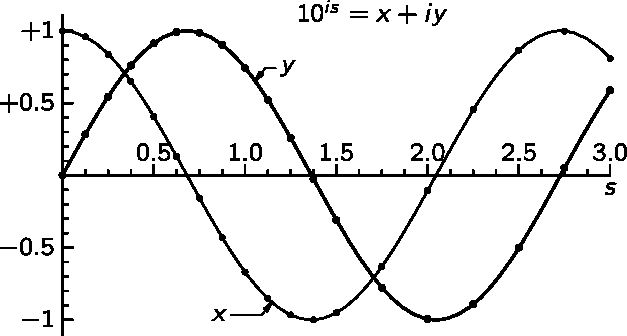
\includegraphics[width=1\linewidth]{fyz_fig0413.pdf}
      \caption{ (\cite[s.~306]{Feynman01})}
      \label{fyz:fig0413}
    \end{figure}

    Tuto kapitolu shrneme nejpozoruhodnějším vztahem matematiky
    \begin{equation}\label{fyz:eq696}
      e^{\imath θ}=\cosθ+\imath\sinθ.
    \end{equation}
    To je náš slibovaný skvost.

    Geometrii můžeme spojit s algebrou tak, že znázorníme komplexní čísla v rovině. Vodorovná poloha
    bodu je \(x\), svislá poloha je \(y\) (obr. \ref{fyz:fig0414}). Tak můžeme zobrazit každé
    komplexní číslo \(x + \imath y\). Nazveme-li radiální vzdálenost bodu \(r\) a úhel
    \(\varTheta\), platí algebraický zákon, že \(x + \imath y\) lze napsat jako re
    \(re^{\imath\varTheta}\), přičemž geometrické vztahy mezi \(x\), \(y\), \(r\) a \(\varTheta\)
    jsou znázorněny na obrázku. Tak vypadá sjednocení algebry a geometrie.

    Je i perioda stejná? Vypočítejme, na jakou mocninu je třeba umocnit \(e\), abychom dostali
    \(i\)? Jaký je logaritmus \(i\) při základu \(e\)? Pro základ \num{10} jsme to již počítali.
    Bylo by to \num{0.68226i}. Když přejdeme k základu \(e\), musíme to vynásobit \num{2.3025}, což
    je \num{1.5709}. Tuto hodnotu budeme nazývat „algebraickým \(\pi/2\)“. Vidíme však, že od
    správné hodnoty \(\pi/2\) se liší jen na posledním desetinném místě, což je způsobeno chybami v
    našich výpočtech! Nejdříve jsme tedy sestrojili čistě algebraickou cestou dvě nové funkce, sinus
    a kosinus, jež patří do algebry a jen do algebry. Nakonec jsme v nich však objevili právě ty
    funkce, s nimiž pracujeme v geometrii, takže mezi algebrou a geometrií zcela určitě existuje
    spojení.

    \begin{figure}[ht!] %\ref{fyz:fig0414}
      \centering
      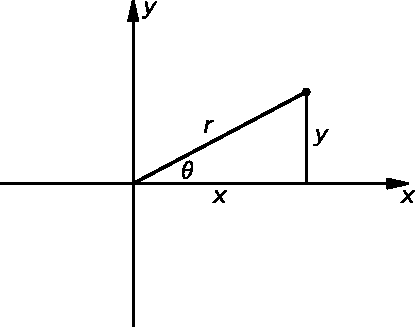
\includegraphics[width=0.9\linewidth]{fyz_fig0414.pdf}
      \caption{Grafické znázornění rovnice \(x + y = re^\imath\) (\cite[s.~306]{Feynman01})}
      \label{fyz:fig0414}
    \end{figure}

    Na začátku této kapitoly, když jsme byli vyzbrojeni jen Základními poznatky o přirozených
    číslech a tím, jak s nimi počítat, neuvědomovali jsme si sílu metody abstrakce a zobecnění.
    Použitím soustavy algebraických „zákonů“ nebo vlastností čísel (\ref{fyz:eq647}) a použitím
    definic inverzních operací (\ref{fyz:eq648}) jsme si sami dokázali vytvořit nejen nové druhy
    čísel, ale rovněž praktické věci, jako jsou tabulky logaritmů, mocnin a trigonometrických funkcí
    (což jsou vlastně imaginární mocniny reálných čísel), a to vše z deseti postupných druhých
    odmocnin desítky.

  \section{Komplexní čísla v Matlabu}\label{fyz:IchapXXIIsecVII}
    Jedna ze zajímavých vlastností Matlabu je možnost práce s komplexními čísly bez další potřebných
    knihoven. Komplexní čísla můžeme zadávat ve složkovém i exponenciálním tvaru. Imaginární
    jednotku zapíšeme jako \(\imath = \jmath = \sqrt{-1}\). Následující výpis obsahuje několik
    příkladů zadání komplexních čísel (\cite[s.~30]{Karban2006}).
    \begin{mdframed}[style=mdmsdos]
      \begin{lstlisting}[style=luaMatlabText,gobble=8]
        % slozkovy tvar - i
        >> c1 = 1-2i 
           c1 = 1.0000 - 2.0000i
        % slozkovy tvar - j
        >> c2 = 2-3j   
           c2 = 2.0000 - 3.0000i
        % exponenciální tvar
        >> c3 = 10*exp(pi/2*i)      
           c3 = 0.0000 + 10.0000i
      \end{lstlisting}
    \end{mdframed} 

    Pro vyjádření imaginární části komplexních čísel lze kromě \(\imath\) použít také \(\jmath\).
    Při počítání s komplexními čísly se také hodí následující funkce:
    \begin{description}
      \item[\texttt{real(c)}]    reálná část.
      \item[\texttt{imag(c)}]    imaginární část
      \item[\texttt{conj(c)}]    komplexní doplněk
      \item[\texttt{abs(c)}]     absolutní hodnota
      \item[\texttt{angle(c)}]   úhel \(\Theta\) v radiánech (obr. \ref{fyz:fig0414}) 
    \end{description}  

    Příkaz \texttt{compass} zobrazí vektory jako šipky směřující od středu souřadnice systému v
    Gaussově rovině:
    \begin{mdframed}[style=mdmsdos]
      \begin{lstlisting}[style=luaMatlabText,gobble=8]
        >> x = [1+0i, -1+0.5i, -0.3-0.4i]
           x = 1.0000 + 0.0000i  -1.0000 + 0.5000i  -0.3000 - 0.4000i
        >> compass(x)
      \end{lstlisting}
    \end{mdframed} 

    \luagraphic[1]{fyz_fig0932.pdf}{Kompasový graf vektorů jako šipek z počátku souřadnic 
      (\cite[s.~91]{Karban2006}}{fyz:fig0932}

  \section{Příklady a cvičení}\label{fyz:IchapXXIIsecVIII}
%---------------------------------------------------------------------------------------------------